%!TEX root=../ast2016.tex

\begin{figure*}[t]
  \centering
  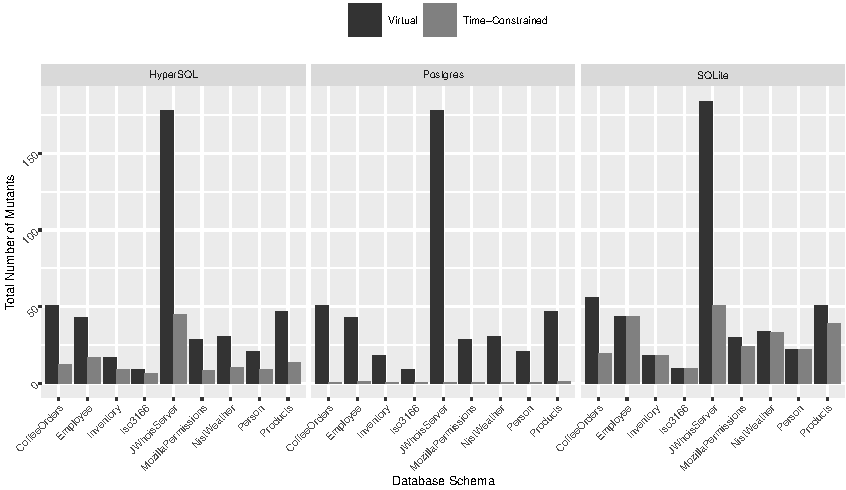
\includegraphics[scale=1.0]{graphics/graphic_barplot_schema_mutationcount_vm_tcm.pdf}
  \caption{Box plot of the mutation score for the virtual and time-constrained mutation analysis techniques.}

  {\small \justifying{\noindent In this plot the box itself represents the interquartile range (IQR), or the measure of
      statistical dispersion that is the difference between the first and third quartiles. Furthermore, the upper
      whisker extends from the top of the box to the highest value that is within 1.5 times the IQR and the lower
      whisker goes from the bottom of the box to the lowest value within 1.5 times the IQR. Finally, the thick
      horizontal line represents the median value, the filled circles denote outliers, and the open diamond is the mean
      value.} \par}

\end{figure*}
